\documentclass{entcs}
\usepackage{entcsmacro}
\usepackage{graphicx}
\usepackage{latexsym}
\usepackage{amssymb}

\def\lastname{Chen AND Wu}
\begin{document}
\begin{frontmatter}

 \title{Model Checking Temporal Aspects of Inconsistent Concurrent Systems Based on Paraconsistent Logic
 }
 \author{Donghuo Chen\thanksref{myemail}},
 \author{Jinzhao Wu$^{1,2}$}
 \address{$^{1}$Chengdu Institute of Computer Applications\\
  Chinese Academy of Sciences, Chengdu 610041, China}
 \address{$^2$Fakult\"at f\"ur Mathematik und Informatik\\
 Universit\"at Mannheim, D7, 27, 68131 Mannheim, Germany}
 \thanks[myemail]{Email:
    \href{mailto:chendonghuo@hotmail.com}{\texttt{\normalshape
        chendonghuo@hotmail.com}}}
%\thanks[ALL]{Partially supported by a NKBRPC (2004CB318000) and by National Science Foundation of China (60373113)}

\begin{abstract}
Classical logic cannot be used to effectively reason about
concurrent systems with inconsistencies (inconsistencies often
occur, especially in the early stage of the development, when large
and complex concurrent systems are developed). In this paper, we
propose the use of a paraconsistent temporal logic (QCTL) for
supporting the verification of temporal properties of such systems
even where the consistent model is not available. We introduce a
novel notion of paraKripke models, which grasps the paraconsistent
character of the entailment relation of QCTL. Furthermore, we
explore the methodology of model checking over QCTL, and describe
the detailed algorithm of implementing QCTL model checker. In the
sequel, a simple example is presented, showing how to exploit the
proposed model checking technique to verify the temporal properties
of inconsistent concurrent systems.
\end{abstract}

\begin{keyword}
inconsistency, concurrent systems, paraconsistent temporal logic,
model checking
\end{keyword}

\end{frontmatter}

\section{Introduction}\label{intro}

In recent years, model checking~\cite{MC} has become an established
technique for automatically verifying the correctness of
finite-state concurrent systems. The technique has been effectively
applied to reasoning about correctness of hardware, communication
protocols, and software engineering, etc.

For the purpose of research and practice, a number of model checkers
have been developed, including SPIN~\cite{spin} and VIS~\cite{VIS}.
Despite their variety, the existing model checkers are typically
based on classical logic, and cannot be therefore used to reason
about the specifications of concurrent systems containing uncertain
or inconsistent information.

To the best of our knowledge, classical logic is very appealing for
formal representation of specifications of concurrent systems and
reasoning due to its expressivity and reasoning power.
Unfortunately, inconsistency causes problems in reasoning with
classical logic. In classical logic, anything can follow from an
inconsistent set of assumptions, that is, inconsistency leads to
trivial and meaningless reasoning. However, it has been figured out
that inconsistency is an unavoidable phenomena in the development of
large and complex concurrent systems~\cite{Incon}. In requirements
engineering, models are frequently inconsistent because they combine
conflicting points of view. During design and implementation,
inconsistency arises when integrating components developed by
different members. A significant proportion of the specification
analysis process is then devoted to detecting and eliminating such
inconsistencies because inconsistencies are traditionally regarded
as undesirable. But from beginning to end, especially at the early
stage, maintaining absolute consistency is not always possible.
Often this is not even desirable since this can unnecessarily
constrain the development process, can lead to the loss of important
information~\cite{Incon1}. Thus, there has been a considerable
amount of research on the development of technique and tools
providing practical support for how to manage inconsistencies in a
more general fashion and possibly reason in the presence of
inconsistencies~\cite{Handle1,Hunter1,Formal}.

Paraconsistent logics and multi-valued
logics~\cite{MVProver1,P.Godefroid}
 provide us with new logical foundations
suited for reasoning under inconsistency.
 Paraconsistent logics~\cite{Para1,Para2}, which are weaker than classical logics
and permit some contradictions to be true, achieve nontrivial
reasoning under inconsistency by non-standard behavior of logical
connectives, by restricting proof systems, and all that. To take
full advantage of paraconsistent logics, developers do not have to
roughly reject system specifications with any inconsistent
information anymore, but analyze them in a more rational fashion.
However, there have been relatively few attempts to develop
automated reasoning tools for inconsistent models at present, and a
majority of work is limited to paraconsistent logics themselves.
Some notable exceptions are Hunter, Nuseibeh, and Riarka
\cite{Hunter1,QZ}, who use a paraconsistent logic QCL to reason
about evolving specifications. Additionally, following the idea of
the paraconsistent logic QCL~\cite{Hunter1}, presented by Hunter, et
al., in this paper we present paraconsistent logic termed QCTL by
extending QCL with the ability to specify the temporal aspects of
concurrent systems. Further, we study the problem of model checking
over the paraconsistent temporal logic QCTL.

The rest of this paper is organized as follow: Section 2 simply
introduces the language of QCTL. Section 3 detailedly discusses the
problem of model checking over QCTL. To motivate our work, Section 4
presents an example, showing the proposed model checking technique
the power of model checking the expected temporal properties of an
inconsistent concurrent system. Section 5 summarizes the paper. For
lack of space, all involved proofs have been
omitted.\section{Paraconsistent temporal logic QCTL} \label{QCTL}

\subsection{Syntax} \label{QCTL:syn}

The syntax of QCTL is that of CTL, but they are very different in
essence. QCTL is based on the paraconsistent logic methodology,
whereas CTL is based on classical propositional logic. This fact
leads to great difference in proof systems and semantics.

Temporary operators are introduced as follows: $\bigcirc$ $-$ at
the next state, $\diamondsuit$ $-$ eventually,  $\Box$ $-$ always,
and  $\texttt{U}$ $-$ until. Moreover, the two path quantifiers
$\texttt{E}$ and $\texttt{A}$ have the intuitive meaning  ``there
is a path" and ``for all paths", respectively.

Let $\mathcal{P}$ denote a set of atomic propositions. Formulas of
QCTL have the following abstract syntax, where $p$ ranges over
$\mathcal{P}$:
\begin{center}
$\alpha:=p\;|\;\neg\alpha\;|\;\alpha_1\wedge\alpha_2\;|\;\alpha_1\vee\alpha_2\;|\;
\texttt{E}(\texttt{A})\bigcirc\alpha\;|\;
\texttt{E}(\texttt{A})\diamondsuit\alpha\;|\;\texttt{E}(\texttt{A})\Box\alpha\;|\;
\texttt{E}(\texttt{A})(\alpha_1\;\texttt{U}\;\alpha_2)$
\end{center}
Let $\mathcal{L}$ denote the set of formulas by the above abstract
syntax. Moreover, $\alpha\rightarrow\beta$ is the abbreviation for
$\neg\alpha\vee \beta$ as usual. Conventionally for each
$p\in\mathcal{P}$, $p$ or $\neg p$ is called a literal. A formula
of the form $l_1\vee\ldots\vee l_n$ for $n\geq 1$ is called a
clause, where $l_1, \ldots, l_n$ are literals. Furthermore, we
provide some basic definitions preparing for the following work.\\

\noindent\textbf{Definition~\ref{QCTL:syn}.1} Such formula in the
form of $\sigma ( \alpha\;\texttt{U}\;\beta)$, $\neg\sigma (
\alpha\;\texttt{U}\;\beta)$, $\sigma\texttt{x}\alpha\mbox{ or
}\neg\sigma\texttt{x}\alpha$ for $\alpha,\beta\in\mathcal{L}$ is
called a quasi-literal, where $\sigma$ represents the path
quantifier $\texttt{E}$ or $\texttt{A}$ and $\texttt{x}$
represents one of the temporal operators
$\bigcirc,\Box,\diamondsuit$. $l_1\vee\ldots\vee\l_n\vee
ql_1\vee\ldots\vee ql_m
  \in\mathcal{L}$ is called a quasi-clause,
where $\forall i. 1\leq i\leq n$, $\l_i$ is a literal and
$\forall i. 1\leq i\leq m$, $ql_i$ is a quasi-literal. Moreover,
a clause or quasi-literal is a special quasi-clause.\\

In the sequel, $\sigma$ and $\texttt{x}$ have the above meaning in
the context, when they are not explicitly interpreted.\\

\noindent\textbf{Definition~\ref{QCTL:syn}.2} Let $F$ be the
smallest set of formulas generated by finitely applying the
following rules:

1. For $p\in\mathcal{P}$, $p,\neg p\in F$.

2. Let $\alpha,\beta\in F$, and $\alpha,\beta$ be two
quasi-clauses, then $\alpha\vee\beta\in F.$

3. For $\alpha,\beta\in F$, $\alpha\wedge \beta\in F$.

4. For $\alpha,\beta\in F$, $\sigma\texttt{x}\alpha,$ $\sigma
(\alpha\;\texttt{U}\;\beta)\in F$.\\


any $\alpha=\alpha_1\wedge\ldots\wedge\alpha_n\in F$ for $n\geq 1$
is called a complete-CNF, and for $1\leq i\leq n$, $\alpha_i$ is
called a complete-clause.

The purpose of defining the set of formulas $F$ is that it helps
us to compute a important set $Fact_s(\alpha)$ for $\alpha\in
\mathcal{L}$ used in implementing the algorithm of model checking
over QCTL, and to establish a concise proof of the completeness of
the proof system for QCTL.

QCTL has the same syntax with the classical temporal logic CTL. It
differs from CTL at the semantic level. This is exactly the point
making QCTL a paraconsistent logic.

\subsection{Semantics}\label{QCTL:sem}

 QCTL is motivated by the need to reason about concurrent systems
with inconsistent specifications. The notion of truth or falsity
is thus discarded. We here view each formula as a belief,
following the idea in~\cite{Hunter1}. QCTL achieves the
paraconsistent methodology by decoupling the relationship between
a formula and its negation at the level of semantics. To reach
this aim, a set of positive and negative objects is first
constructed from the set $\mathcal{P}$ of atomic propositions. For
each $p\in\mathcal{P}$, $+p$ is called a
positive object and $-p$ a negative object.\\

\noindent\textbf{Definition~\ref{QCTL:sem}.1}  The set of positive
and negative objects in QCTL is defined as
$\mathcal{O}=\{+p\;|\;p\in
\mathcal{P}\}\cup\{-p\;|\; p\in\mathcal{P}\}.$ \\

Kripke structures are widely used as semantic models of temporal
logics such as CTL \cite{kri1}. We here provide QCTL with a novel
semantics by extending Kripke structures to
paraKripke structures. \\

\noindent\textbf{Definition~\ref{QCTL:sem}.2} A tuple $M=(S,R,L)$
is called a paraKripke structure, where
\begin{itemize}
\item ${S}$ is a non-empty state set. \item ${R\subseteq S\times
S}$ is a total relation, which implies for each $s\in S$ there
exists $t\in S$ satisfying $(s,t)\in R$. \item ${L:S\mapsto
2^{\mathcal{O}}}$ is a label function, which labels each state
with a set of the positive or negative objects.
\end{itemize}
ParaKripke structures are similar to the general Kripke structures
except for the label functions. But it is the label function that
grasps the essential idea behind the structures. In a paraKripke
structure, the states are labeled by positive or negative objects
included in $\mathcal{O}$.
ParaKripke structures will be used as the semantic model of QCTL.\\

\noindent\textbf{Definition~\ref{QCTL:sem}.3} Let $M=(S,R,L)$ be a
paraKripke structure. A computing path $x$ of $M$ is defined as
$x=(s_1, \ldots, s_i, \ldots)$, where for all $i\geq 1$, $s_i\in
S$ and $(s_i,s_{i+1})\in R$. $s_1$ is called the initial state of
$x$, and $(s_1,\ldots,s_k)$ for $k\ge 1$ an initial
prefix of $x$. \\

Before defining the satisfiability relation in QCTL, we first
present the satisfiability notion of a literal belief in a state.
For a paraKripke structure $M=(S,R,L)$, let $s\in S$, $E_s=L(s)$
and $p\in\mathcal{P}$. Then (1) $p$ is satisfiable in $s$ iff
$+p\in E_s$, and (2) $\neg p$ is satisfiable in $s$ iff $-p\in
E_s$.

From the above discussion, we see that paraKripke structures
incorporate the notion of belief, in which it is possible that both
an atomic proposition and its negation are satisfiable in a same
state, that is, a state can be labeled by $+p \mbox{ and }-p $ for
$p\in\mathcal{P}$. Therefore, QCTL decouples the link between a
formula and its negation at the level of semantics. This makes it a
paraconsistent logic.

For achieving the non-trivial inference under inconsistencies, a
proof procedure in QCTL is a two-stage affair: decompositional
steps followed by compositional steps, by which the trivial
reasoning is avoided under inconsistency. The details can be found
in the full vision of the paper. To capture this idea, we need to
establish two satisfiability relations for both stages called the
strong satisfiability relation and the weak satisfiability
relation. The notion of strong satisfaction corresponds to the
decompositional phase and the notion of weak satisfaction
corresponds to the compositional phase, respectively.\\

\noindent\textbf{Definition~\ref{QCTL:sem}.4} Let $M=(S,R,L)$ be a
paraKripke structure. The strong satisfiability relation
$\models_{ts}$ is defined as follows:

 1. For atomic formula $p$, $(M,s)\models_{ts} p  \mbox{ iff } +p\in L(s)$.

 2. For atomic formula $p$, $(M,s)\models_{ts} \neg p\mbox{ iff }
-p\in L(s)$.

 3. $(M,s)\models_{ts} \alpha\wedge\beta\mbox{ iff }
(M,s)\models_{ts}\alpha \mbox{ and } (M,s)\models_{ts}\beta$.

 4. For a clause
 $\alpha=l_1\vee\ldots\vee l_n$, where
 $l_1,\ldots,l_n$ are literals,
 $(M,s)\models_{ts}\alpha$ iff $\exists i.1\le i\le n,$
 $(M,s)\models_{ts}l_i$ and $\forall i.1\leq i\leq n$, $(M,s)\models_{ts} \neg
l_i$ implies $(M,s)\models_{ts} Disj(\alpha,l_i)$, where
$Disj(\alpha,l_i)$ is the original formula $l_1\vee\ldots\vee l
_n$ without the disjunct $l_i$.

 5. For a quasi-clause $\alpha=l_1\vee\ldots\vee l_n\vee
  ql_1\vee\ldots\vee ql_m$, $(M,s)\models_{ts} \alpha\mbox{ iff }
 (M,s)\models_{ts}l_1\vee\ldots\vee l_m
\mbox{ or } \exists i.1\le i\le m,$ $(M,s)\models_{ts} ql_i$,
where $l_1,\ldots,l_n$ are literals, and $ql_1,\ldots,ql_m$ are
quasi-literals.

6. $(M,s)\models_{ts}\texttt{E}\bigcirc \alpha$ iff there is
 $t\in S$ satisfying $(s,t)\in R$ and $(M,t)\models_{ts} \alpha$.


 7. $(M,s)\models_{ts}\texttt{A}\bigcirc \alpha$ iff  for all $t\in
 S$ with $(s,t)\in R$, $(M,t)\models_{ts} \alpha$.


8. $(M,s)\models_{ts}\texttt{E}\diamondsuit\alpha$ iff there
 is a computing path $x=(s_0, \ldots, s_n, \ldots)$ with $s_0=s$ and
$\exists i.i\geq 1$, $(M,s_i)\models_{ts}\alpha$.% \item


9. $(M,s)\models_{ts} \texttt{A}\diamondsuit\alpha$ iff for all
computing paths with initial state $s$, $(M,s)\models_{ts}
\texttt{E}\diamondsuit\alpha $.

10. $(M,s)\models_{ts} \texttt{E}(\alpha\;\texttt{U}\;\beta)$ iff
there is an initial prefix $(s_0, \ldots, s_k)$ of a computing
path $x$
 with the initial state $s_0=s$, satisfying that $(M,s_k)\models_{ts} \beta$ and
$(M,s_i)\models_{ts} \alpha$ for all $i<k$.

11. $(M,s)\models_{ts}\texttt{A}(\alpha\;\texttt{U}\; \beta)$ iff
for all computing paths with initial state $s$,
$(M,s)\models_{ts}\texttt{E}(\alpha\;\texttt{U}\;\beta)$. %\item

12. $(M,s)\models_{ts}\texttt{E}\Box \alpha$ iff there is a
computing path $x=(s_0, \ldots, s_n,\ldots)$ with $s_0=s$ and
$\forall i.i\geq 0$, $(M,s_i)\models_{ts}\alpha$.

13. $(M,s)\models_{ts}\texttt{A}\Box \alpha$ iff for each
computing path $x=(s_0, \ldots, s_n, \ldots)$ with the initial
state $s_0=s$, $(M,s_i)\models_{ts}\alpha$, where $i\geq 0$.\\


\noindent\textbf{Definition~\ref{QCTL:sem}.5}  The weak
satisfiability relation $\models_{tw}$ is defined as follows:
\begin{itemize}
\item In all the items except for the fourth  in
Definition~\ref{QCTL:sem}.4,
 $\models_{ts}$ is replaced by $\models_{tw}$.
\item For a clause $\alpha=l_1\vee\ldots\vee l_n$,
$(M,s)\models_{tw} \alpha \mbox{ iff } \exists i.1\le i\le n,
 (M,s)\models_{tw}l_i$.
\end{itemize}

The strong satisfiability is much more restricted than the weak
satisfiability relation with regard to disjunction, as shown in
the fourth and fifth items of Definition~\ref{QCTL:sem}.4. The
reason we need such motivation is that we have decoupled the link
between a formula and its negation. By putting the link between
each disjunct in a quasi-clause and its negation into the
definition for disjunction, we, on the one hand, to some degree
provide the meaning of negation operator $\neg$, on the other
hand, provide a semantics account for paraconsistent reasoning
using resolution.

Clearly, the strong and weak satisfiability relations do not cover
all formulae in $\mathcal{L}$, For instance,
$\alpha\wedge(\beta\vee\gamma)$ and $\neg\texttt{E}\diamondsuit
\alpha$, where $\alpha,\beta,\gamma\in\mathcal{L}$, therefore we
need to extend Definition~\ref{QCTL:sem}.4 and~\ref{QCTL:sem}.5.
Before accomplishing this work, we define a binary relation
$\approx_t$ on $\mathcal{L}$.\\

\noindent\textbf{Definition~\ref{QCTL:sem}.6} Let $\alpha,\beta\in
\mathcal{L}$. $\alpha \approx_t \beta$ iff for every paraKripke
structure $M=(S,R,L)$ and every $s\in S$,
$(M,s)\models_{ts}\alpha$ ($(M,s)\models_{tw}\alpha$) implies
$(M,s)\models_{ts}\beta$
(respectively, $(M,s)\models_{tw}\beta$), and vice versa.\\

\noindent\textbf{Proposition~\ref{QCTL:sem}.1} $\approx_t$ is an
equivalence
relation on $\mathcal{L}$. \\

For defining full semantics of QCTL, we make the strong and weak
satisfiability relations cover all formulae in $\mathcal{L}$ by
extending Definition~\ref{QCTL:sem}.4 and~\ref{QCTL:sem}.5. The
strong and weak satisfiability models of formulae of the form
$\neg\sigma\texttt{x}\alpha$ and $\neg\sigma(\alpha\ \texttt{U}\
\beta)$ can be indirectly defined as E'1-E'6 by $\approx_t$. In a
similar way, we further define the full behavior of
$\neg,\vee,\mbox{ and }\rightarrow$ as E1-E7 in order that the
strong and weak satisfiability relations cover all formulas in
$\mathcal{L}_t$.


E1. $\neg\neg \alpha\vee \beta \approx_t \alpha\vee \beta\qquad
\qquad\qquad\ \ \ \ \ $ E'1.
$\neg\texttt{E}\bigcirc\alpha\approx_t\texttt{A}\bigcirc(\neg
\alpha) $
%\item []

E2. $\neg (\alpha\wedge \beta)\vee \gamma
\approx_t\neg \alpha\vee\neg \beta\vee \gamma \qquad\ \ $ E'2.
$\neg\texttt{A}\bigcirc \alpha\approx_t\texttt{E}\bigcirc (\neg
\alpha)$ %\item []

E3. $\neg(\alpha\vee \beta)\vee \gamma\approx_t (\neg
\alpha\wedge\neg \beta)\vee \gamma\quad\ \ \ \ $E'3. $\neg
\texttt{E}\diamondsuit \alpha\approx_t\texttt{A}\Box (\neg \alpha)
$ %\item[]

E4. $\alpha\vee(\beta\wedge\gamma)\approx_t (\alpha\vee
\beta)\wedge (\alpha\vee \gamma)\quad\ \;$ E'4. $\neg
\texttt{A}\diamondsuit \alpha\approx_t\texttt{E}\Box(\neg \alpha)$
%\item []

E5. $\alpha\wedge (\beta\vee \gamma)\approx_t (\alpha\wedge
\beta)\vee (\alpha\wedge \gamma)\ \ \ \ \ $ E'5.
$\neg\texttt{E}(\alpha\; \texttt{U}\; \beta)\approx_t
\texttt{A}\Box(\neg \beta)\vee\texttt{A}((\alpha$

$\qquad\qquad\qquad\qquad\qquad\qquad\qquad\qquad\qquad\ \ \
\wedge \neg \beta )\texttt{U}(\neg \alpha\wedge\neg \beta))$
%\item[]

E6. $(\alpha\rightarrow \beta)\vee \gamma \approx_t \neg
\alpha\vee \beta\vee \gamma\qquad\qquad$ E'6. $\neg
\texttt{A}(\alpha\; \texttt{U}\;
\beta)\approx_t\texttt{E}\Box(\neg \beta)\vee\texttt{E}((\alpha$

$\qquad\qquad\qquad\qquad\qquad\qquad\qquad\qquad\qquad\ \
\wedge\neg \beta )\texttt{U}(\neg \alpha\wedge\neg \beta))$
%\item[]

E7. $\neg (\alpha\rightarrow \beta)\vee \gamma\approx_t
(\alpha\wedge\neg \beta)\vee \gamma$

So far, we have made all preparations for defining the entailment
relation $\models_t$ of QCTL. Let $2^{\mathcal{L}}$
denote the power set of $\mathcal{L}$:\\

\noindent\textbf{Definition~\ref{QCTL:sem}.7} The entailment
relation $\models_{t}$ of QCTL is defined as follows:
\begin{itemize}
\item $\models_t \subseteq (2^{\mathcal{L}}-\emptyset)\times
\mathcal{L}$, where $\emptyset$ is the empty set. \item For
$\Gamma\in 2^{\mathcal{L}}-\emptyset$ and $\beta\in \mathcal{L}$,
$\Gamma\models_t \beta$ iff for all paraKripke structure
$M=(S,R,L)$ and $s\in S$, $(M,s)\models_{ts}\alpha$ for all
$\alpha\in\Gamma$ implies $(M,s)\models_{tw}\beta$.
\end{itemize}

The entailment relation is paraconsistent. In the next section, we
will build the novel notion of model based on the entailment
relation $\models_t$, such that we can employ automatically model
checking technique to analyze the temporal properties of concurrent
systems in the presence of inconsistency.

\section{QCTL model checking}\label{mc}

\subsection{Methodology}\label{MC:metho}

As mentioned above, we can model concurrent systems containing
inconsistent information using paraKripke structures. Because the
entailment relation $\models_t$ of QCTL is defined in a mode, very
different from that of classical logic, it is unapt for paraKripke
structures to model specifications of inconsistent concurrent
systems, just as standard Kripke structures do in~\cite{MC,TL}.

In what follows, we build the notion of models based on paraKripke
structures, which differs from that based on standard Kripke structures.\\

\noindent\textbf{Definition~\ref{MC:metho}.1} Let
 $\alpha\in\mathcal{L}$, and a tuple $M=(S,R,L,S_0)$ be a paraKripke
 structure, where $S_0\subseteq S$ is a non-empty set of initial
 states. $(M,s_0)\models_t\alpha$ for $s_0\in S_0$ iff there
 exists a finite set of formulas $\Gamma\subseteq\mathcal{L}$,
 which satisfies that $\forall\gamma.\gamma\in\Gamma$,
 $(M,s_0)\models_{ts}\gamma$ and $\Gamma\models_t\alpha$. $M$ is a
 paraKripke model of $\alpha$ iff $\forall s.s\in S_0$,
 $(M,s)\models_t\alpha$.\\

 We argue that it is unaccepted to directly transform a model checking
problem to an inference problem according to
Definition~\ref{MC:metho}.1. Hence, the following work focuses our
efforts on studying the method of performing model checking over
QCTL.

Many assertions, which naturally hold in classical model checking
method, are not evident, even completely improper in the case of
model checking over QCTL, i.e., typically, for a temporal formula
$\alpha$ in CTL, a model of $\alpha$ implies that it is not a
model of $\neg\alpha$.

Given a paraKripke structure $M=(S,R,L,S_0)$, we first provide
some basic propositions.\\

\noindent\textbf{Proposition~\ref{MC:metho}.1} Let
$l_1,\ldots,l_n$ for $n\geq 1$ be literals, and $ql_1,\ldots,ql_m$
for $m\geq 1$ quasi-literals. For $s\in S$,

1. $(M,s)\models_t l_1\vee\ldots\vee l_n $ iff $(M,s)\models_t
l_1$ or $\ldots$ or $(M,s)\models_t l_n$.

2. $(M,s)\models_t l_1\vee\ldots\vee l_n\vee ql_1\vee\ldots\vee
ql_m$ iff $(M,s)\models_t l_1\vee\ldots\vee l_n$, $(M,s)\models_t
ql_1$ or $\ldots$ or $(M,s)\models_t ql_m$.\\

\noindent\textbf{Proposition~\ref{MC:metho}.2} Let
$\alpha,\beta\in\mathcal{L}$. For $s\in S $,

1. $(M,s)\models_t\alpha\vee\beta$ iff $(M,s)\models_t\alpha$ or
$(M,s)\models_t\beta$.

2. $(M,s)\models_t\alpha\wedge\beta$ iff $(M,s)\models_t\alpha$
and $(M,s)\models_t\beta$.

3. Let
$\alpha_1\wedge\ldots\wedge\alpha_n$ for $n\geq 1$ be a
complete-CNF
 of $\alpha$. $(M,s)\models_t\alpha$ iff
$(M,s)\models_t\alpha_1$ and $\ldots$ and
$(M,s)\models_t\alpha_n$.\\

Proposition~\ref{MC:metho}.2 does not mean that
$\Gamma\models_t\alpha\vee\beta$ must result in
$\Gamma\models_t\alpha$ or $\Gamma\models_t\beta$. Consider
$\Gamma=\{p\vee q\}$ for $p,q\in\mathcal{P}$. Obviously,
$\Gamma\models_t p\vee q$, but $\Gamma\not\models_t p$ and
$\Gamma\not\models_t q$.

For a formula $\alpha$, Let
$Fact_s(\alpha)=\{\alpha'\;|\;(M,s)\models_{ts}\alpha'\mbox{
implies }(M,s)\models_{tw}\alpha\}$,
 intuitively called a set of
strong factors of $\alpha$. The detailed definition of
$Fact_s(\alpha)$ will be postponed until the next subsection.\\

\noindent\textbf{Proposition~\ref{MC:metho}.3} Let
$\alpha\in\mathcal{L}$, and $s\in S$. The followings hold:
%\begin{itemize}

1. $(M,s)\models_t\texttt{E}\bigcirc\alpha$ iff $\exists t.t\in S,
(s,t)\in R\mbox{ and }(M,t)\models_t\alpha$.

2. $(M,s)\models_t\texttt{E}\diamondsuit\alpha$ iff there is a
computing path $(s_0,s_1,\dots)$ with the initial state $s_0=s$,
satisfying that $\exists i.i\geq 1$, $(M,s_i)\models_t\alpha$.\\

We have derived some basic conclusions on paraKripke models, which
are the base of implementing the detailed algorithms. But so far,
we do not involve the method of model checking these formulas,
such as $\texttt{E}(\alpha\;\texttt{U}\;\beta)$,
$\texttt{A}\Box\alpha$ and $\texttt{A}\bigcirc\alpha$ for
$\alpha,\beta\in\mathcal{L}$. The paraconsistent character of the
entailment relation of QCTL makes model checking these formulas
more complex and more intractable than $\texttt{E}\bigcirc\alpha$
and $\texttt{E}\diamondsuit\alpha$.

Now take a look at $\texttt{E}(\alpha\;\texttt{U}\;\beta)$.
According to Definition~\ref{MC:metho}.1, for $s\in S$,
$(M,s)\models_t\texttt{E}(\alpha\;\texttt{U}\;\beta)$ means that
$\exists
\Gamma.\Gamma\subseteq\mathcal{L},\forall\gamma.\gamma\in\Gamma,(M,s)\models_{ts}\gamma$
and $\Gamma\models_t\texttt{E}(\alpha\;\texttt{U}\;\beta)$. The
proof system for QCTL determines there must exist
$\texttt{E}(\alpha'\;\texttt{U}\;\beta')$, satisfying that
$\texttt{E}(\alpha'\;\texttt{U}\;\beta')\in\Gamma$, or that
$\texttt{E}(\alpha'\;\texttt{U}\;\beta')$ is derived from $\Gamma$
by applying the decompositional rules, where $\alpha'\in
Fact_s(\alpha)$ and $\beta'\in Fact_s(\beta)$. In other words,
$(M,s)\models_t\texttt{E}(\alpha\;\texttt{U}\;\beta)$
 iff $(M,s)\models_{ts}\texttt{E}(\alpha'\;\texttt{U}\;\beta').$
 According
to the traditional viewpoint,
$(M,s)\models_t\texttt{E}(\alpha\;\texttt{U}\;\beta)$ iff there
exists some initial prefix $(s_0,\ldots,s_k)$ of a computing path
with the initial state $s_0=s$, satisfying that
$(M,s_k)\models_t\beta$ and $(M,s_i)\models_t\alpha$ for $0\leq
i<k$. However, this verdict is not correct in the notion of
paraKripke models.

Let us illustrate this point by an example. Fig.1 show a
paraKripke structure $M$ with the initial state $s_0$, where
$L(s_0)=\{+p,-q,-r,-p'\}$,$L(s_1)=\{-p,+q,-r,-p'\}$,
$L(s_2)=\{-p,-q,+r,-r,-p'\}$ and $L(s_3)=\{-p,-q, +r,+p'\}$ for
$p,q,r,p'\in\mathcal{P}$.
\begin{figure}
\centering\includegraphics{example.eps} \caption{An example of
paraKripke model} \label{fig:model}
\end{figure}

Consider the temporal property $\texttt{E}(p\vee q\vee
r\;\texttt{U}\;p')$. Clearly, for $0\leq i\leq 2$,
$(M,s_i)\models_{t} p\vee q\vee r$, and $(M,s_3)\models_t p'$. But
it cannot educe $(M,s_0)\models_t\texttt{E}(p\vee q\vee
r\;\texttt{U}\;p')$. In fact, $Fact_s(p\vee q\vee r)=\{p,q,r,p\vee
q,p\vee r,q\vee r,p\vee q\vee r \}$. From Fig.1, we see that there
is not any $f_s\in Fact_s(p\vee q\vee r)$, satisfying that for
$0\leq i\leq 2$, $(M,s_i)\models_{ts}f_s$, in other words,
$(M,s_0)\not\models_{t}\texttt{E}(p\vee q\vee r\;\texttt{U}\;p')$.

Similarly, model checking such formulas beginning with the
universal quantifier $\texttt{A}$ and $\texttt{E}\Box\alpha$ faces
the same challenge like model checking
$\texttt{E}(\alpha\;\texttt{U}\;\beta)$: the paraconsistency of
the entailment relation increases the complexity of model checking
such formulas.

ParaKripke structures weaken the  meaning of negation operator
$\neg$ in the sense that both $\alpha$ and $\neg\alpha$ are
exclusively satisfied each other. In model checking over QCTL,
$(M,s)\models_t\alpha$ does not deny $(M,s)\models_t\neg\alpha$.
Hence, the problem of model checking formulas, such as
$\neg\alpha$ and $\neg\texttt{E}\diamondsuit\alpha$, has to be
solved in term of the behavior of the negation operator $\neg$ in
paraPkripke models. Take some examples as follows:
$(M,s)\models_t\neg(\alpha\vee\beta)$ iff
$(M,s)\models_t\neg\alpha\wedge\neg\beta$,
$(M,s)\models_t\neg\texttt{E}\diamondsuit\alpha$ iff
$(M,s)\models_t\texttt{A}\Box(\neg\alpha)$, and
$(M,s)\models_t\neg(\alpha\rightarrow\beta)$ iff
$(M,s)\models_t\alpha\wedge\neg\beta$.

\subsection{Implementing the algorithm}\label{MC:algo}

The model checking problem for QCTL is to verify for a given
paraKripke structure $M$, a state $s\in S$, and a formula
$\alpha\in\mathcal{L}$ whether $(M,s)\models_t\alpha$. Though QCTL
is a paraconsistent temporal logic, we can basically implement the
algorithm in spirit that is inspired by~\cite{ALG1}. This point
gets demonstrated just by what the last subsection gives.

Before deep analyzing the algorithm given in Fig.2, we now provide
the more accurate interpretation of the aforementioned set
$Fact_s(\alpha)$ for $\alpha\in\mathcal{L}$, which is vital for
constructing the algorithm. For a clause $\alpha\in\mathcal{L}$,
let $Literals(\alpha)=\{ l\; |\; l\mbox{ is a disjunct of
}\alpha\}$. The following definition specifies
$Fact_s(\alpha)$ in the case of a complete-clause $\alpha$.\\

\noindent\textbf{Definition~\ref{MC:algo}.1} Let $\alpha$ be a
complete-clause. $Fact_{s}(\alpha)$ is inductively defined as
follows:\small
\begin{itemize}
\item If $\alpha=l_1\vee\ldots\vee l_n$ for $n\geq 1$ is a clause,
then $Fact_s(\alpha)=\bigcup\limits_{i=1}^n\{ l_1\vee\ldots\vee
l_i\; |\; Literals(l_1\vee\ldots\vee l _i)\subseteq
Literals(\alpha) \}$. \item If
$\alpha=\sigma\texttt{x}(\beta_1\wedge\ldots\wedge \beta_n)$, then
$Fact_s(\alpha)=\{\sigma\texttt{x}(\beta'_1\wedge\ldots\wedge
\beta'_n)\; |\; \mbox{for }1\leq i\leq n, \beta'_i \in
Fact_s(p_i)\}$. \item If $\alpha=\sigma((\beta_1\wedge\ldots\wedge
\beta_n)\ \texttt{U}\ (\gamma_1\wedge\ldots\wedge \gamma_m))$,
then $Fact_s(\alpha)= \{\sigma((\beta'_1\wedge\ldots\wedge
\beta'_n)\ \texttt{U}\ (\gamma'_1\wedge\ldots\wedge \gamma'_m))\;
|\; \mbox{for }1\leq i\leq n \mbox{ and }1\leq j\leq m,
\beta'_i\in Fact_s(\beta_i),\gamma'_j\in Fact_s(\gamma_j)\}$.
\item If $\alpha=l_1\vee\ldots\vee ql_i\vee\ldots\vee ql_n$, where
for $i\leq j\leq n$, $ql_j$ is a quasi-literal, and if $i>1$, for
$1\leq j\leq i-1$, $l_j$ is a literal, then
$Fact_s(\alpha)=\bigcup\limits_{m=1}^n\{
\gamma_1\vee\ldots\vee\gamma_m\; |\; \mbox{for }1\leq l\leq
m,\mbox{if $\gamma_l$ is a quasi-literal, } \gamma_l\in
Fact_s(ql_i)\cup \ldots\cup Fact_s(ql_n),\mbox{ and if $\gamma_l$
is a literal, }\exists k.1\leq k<i, \gamma_l=l_k\}$.
\end{itemize}\normalsize
So for any formula $\alpha\in\mathcal{L}$, let
$\alpha_1\wedge\ldots\wedge\alpha_n$ for $n\geq 1$ be the
complete-CNF of $\alpha$.
$Fact_s(\alpha)=\{\alpha_1'\wedge\ldots\wedge\alpha_n'\;|\;\mbox{for
}1\leq i\leq n,\alpha_i'\in Fact_s(\alpha_i) \}$.\\

Fig.2 and Fig.3 show the details of the naive algorithm for model
checking over QCTL. In fact, the function Check($\alpha$) returns
the set of states denoted $Sat(\alpha)$, in which the property
$\alpha$ is satisfied, that is, for $s\in Sat(\alpha)$,
$(M,s)\models_t\alpha$. $Sat(\alpha)$ is computed in a recursive
way by considering the sub-formulas of $\alpha$, similarly like
what has been done in~\cite{TL}. The recursive computation
basically boils down to a bottom-up traversal of the parse tree of
the formula $\alpha$. Each node of the parse tree of $\alpha$
represents a sub-formula of $\alpha$, and the only root node
represents the formula $\alpha$. But because paraKripke structures
decouple the relationship between a formula and its negation at
the level of semantics and the notion of paraKripke models is
introduced, involving the strong satisfiability relation, the
parse tree of a formula is constructed in a different means from
the traditional method, namely, the set of sub-formulas of a
formula has different underlying meaning.
\begin{figure}[htbp]
\centering\scriptsize{\framebox{
\parbox{10cm}{
\textbf{function} CheckEU($\alpha,\Phi$: formula): set of states;\\
\textbf{begin}\\
$\mbox{}\ \ \ \ $ \textbf{var} satpsi, now, pre, sat: set of states\\
$\mbox{}\ \ \ \ $ satpsi, now, pre, sat$f_s$, sat=Check($\Phi$), $\emptyset$, $\emptyset$, $\emptyset$, $\emptyset$ \\
$\mbox{}\ \ \ \ $ \textbf{for} each $f_s\in Fact(\alpha)$\\
$\mbox{}\ \ \ \ \ \ \ \ \ $ sat$f_s$=CheckS($f_s$)\\
$\mbox{}\ \ \ \ \ \ \ \ \ $ now=satpsi\\
$\mbox{}\ \ \ \ \ \ \ \ \ $ \textbf{do}\\
$\mbox{}\ \ \ \ \ \ \ \ \ \ \ $ pre=now\\
$\mbox{}\ \ \ \ \ \ \ \ \ \ \ $ now=pre $\cup$
($\{s\;|\;R(s)\cap\mbox{pre}\neq\emptyset \}\cap\mbox{ sat$f_s$}$)

 $\mbox{}\ \ \ \ \ \ \ \ \ $ \textbf{until} pre=now\\
$\mbox{}\ \ \ \ \ \ \ \ \ $ sat=sat $\cup$ now

$\mbox{}\ \ \ \ $ \textbf{end for}\\
$\mbox{}\ \ \ \ $ \textbf{return} sat

\textbf{end}\\


\textbf{function} CheckEG($\alpha$: formula): set of states;\\
\textbf{begin}\\
$\mbox{}\ \ \ \ $ \textbf{var} satpsi, now, pre, sat: set of states\\
$\mbox{}\ \ \ \ $ satpsi, now, pre, sat$f_s$, sat=Check($\Psi$),
S,
$\emptyset$, $\emptyset$, $\emptyset$\\
$\mbox{}\ \ \ \ $ \textbf{for} each $f_s\in Fact(\Psi)$\\
$\mbox{}\ \ \ \ \ \ \ \ \ $ sat$f_s$=CheckS($f_s$)\\
$\mbox{}\ \ \ \ \ \ \ \ \ $ now=$S$\\
$\mbox{}\ \ \ \ \ \ \ \ \ $ \textbf{do}\\
$\mbox{}\ \ \ \ \ \ \ \ \ \ \ $ pre=now\\
$\mbox{}\ \ \ \ \ \ \ \ \ \ \ $ now=pre $\cap$ ($\{s\in S\;|\;R(s)\cap\mbox{pre}\neq\emptyset\}\cap\mbox{sat$f_s$}$)\\
$\mbox{}\ \ \ \ \ \ \ \ \ $ \textbf{until} now=pre\\
$\mbox{}\ \ \ \ \ \ \ \ \ $ sat=sat $\cup$ now\\
$\mbox{}\ \ \ \ $ \textbf{end for}\\
$\mbox{}\ \ \ \ $ \textbf{return} sat

\textbf{end}\\


\textbf{function} Check($\alpha$: formula):
set of states ;\\
\textbf{begin} \\
\noindent$\mbox{  }\ \ \ \ $ \textbf{switch}($\alpha$)\\
 $\mbox{}\ \ \ \ \ \ \ \ \ $ \textbf{case} $\alpha=p\in\mathcal{P}$: \textbf{return} $\{s\;|\;s\in S,+p\in L(s)\}$\\
 $\mbox{}\ \ \ \ \ \ \ \ \ $ \textbf{case} $\alpha=\neg p$ for $p\in\mathcal{P}$:
\textbf{ return }$\{s\;|\;s\in S,-p\in L(s)\}$\\
 $\mbox{}\ \ \ \ \ \ \ \ \ $ \textbf{case} $\alpha=\alpha_1\wedge\alpha_2$:
 \textbf{return}
 Check($\alpha_1$) $\cap$ Check($\alpha_2$)\\
 $\mbox{}\ \ \ \ \ \ \ \ \ $ \textbf{case} $\alpha=\alpha_1\vee\alpha_2$:
 \textbf{return}
 Check($\alpha_1$) $\cup$ Check($\alpha_2$)\\
 $\mbox{}\ \ \ \ \ \ \ \ \ $ \textbf{case} $\alpha=\texttt{E}\bigcirc\alpha_1$:
\textbf{ return} $\{s\in
 S\;|\;R(s)\cap\mbox{Check($\alpha_1$)}\neq\emptyset\}$\\
 $\mbox{}\ \ \ \ \ \ \ \ \ $ \textbf{case}
 $\alpha=\texttt{E}(\alpha_1\;\texttt{U}\;\alpha_2)$:
 \textbf{return}
 CheckEU($\alpha_1,\alpha_2$)\\
 $\mbox{}\ \ \ \ \ \ \ \ \ $ \textbf{case} $\alpha=\texttt{E}\Box\alpha_1$:
 \textbf{return}
 CheckEG($\alpha_1$)\\
 $\mbox{}\ \ \ \ \ \ \ \ \ $ \textbf{case}
 $\alpha=\neg(\alpha_1\wedge\alpha_2)$: \textbf{return}
 Check($\neg\alpha_1\vee\neg\alpha_2$)\\
$\mbox{}\ \ \ \ \ \ \ \ \ $ \textbf{case}
$\alpha=\neg\texttt{E}\diamondsuit\alpha_1$: \textbf{return}
Check($\texttt{A}\Box\alpha_1$)\\
$\mbox{}\qquad \qquad \qquad\vdots$

\noindent$\mbox{  }\ \ \ \ $ \textbf{end switch}

\textbf{end}
 }}}
 \caption{The recursive algorithm for model checking over QCTL}
 \label{fig:ALG}
\end{figure}

\begin{figure}[htbp]

\centering\scriptsize{ \fbox{
\parbox{10cm}{
\textbf{function} TestClause($s$: state, $c$: clause): True or
False;\\
$\mbox{}\ \ \ \ \ $($^\ast c=c_1\vee\ldots\vee c_n$ for $n\geq
1^\ast$)

\textbf{begin}\\
\noindent$\mbox{  }\ \ \ \ $ \textbf{if} $n=1$ return (+$c_1\in
L(s)$ ? True : False)\\
\noindent$\mbox{  }\ \ \ \ $ \textbf{else}\\
\noindent$\mbox{  }\ \ \ \ \ \ \ $ \textbf{if} $+c_1\not\in
L(s)\ldots\mbox{and}+c_n\not\in L(s)$ \textbf{return} False\\
\noindent$\mbox{  }\ \ \ \ \ \ \ $ \textbf{for} $1\leq i\leq n$\\
\noindent$\mbox{  }\ \ \ \ \ \ \ \ \ $ \textbf{if} $+c_i\in
L(s)$\\
\noindent$\mbox{  }\ \ \ \ \ \ \ \ \ \ \ $ \textbf{if}
TestClause(s, $Disj(c,c_i))=\mbox{False}$ \textbf{return} False


\noindent$\mbox{  }\ \ \ \ \ \ \ $ \textbf{end for}\\
\noindent$\mbox{  }\ \ \ \ \ \ \ $ \textbf{return} True

\textbf{end}\\


\textbf{function} CheckS($\alpha$: complete-CNF formula): set of
states;\\
$\mbox{}\ \ \ \ \ $($^\ast\alpha=\alpha_1\wedge\ldots\wedge\alpha_n \mbox{ for }n\geq 1 ^\ast$)\\
\textbf{begin}\\
\noindent$\mbox{  }\ \ \ \ $ \textbf{if} $n>1$ \textbf{return}
$\bigcap\limits_{i=1}^n$CheckS($\alpha_i$)\\
$\mbox{  }\ \ \ \ $ \textbf{else}\\
$\mbox{}\ \ \ \ \ \ \ \ $ \textbf{switch}$(\alpha)$\\
$\mbox{ }\ \ \ \ \ \ \ \ \ \ \ $ \textbf{case}
$\alpha=l_1\vee\ldots\vee\l_m$: \textbf{return}
$\{s\;|\;\mbox{TestClause}(s,\alpha)=\mbox{True}\}$ \\
$\mbox{}\ \ \ \ \ $($^\ast
m\geq 1 $ and for $1\leq i\leq m$, $l_i$ is a literal.$^\ast$)\\
$\mbox{ }\ \ \ \ \ \ \ \ \ \ \ $ \textbf{case} $\alpha=c\vee
ql_1\vee\ldots\vee ql_m$: \textbf{return}
CheckS($c$)$\cup$CheckS($ql_1$)\\$\cup\ldots\cup$CheckS($ql_m$)
($^\ast m\geq 1 $, and for $1\leq i\leq m$, $ql_i$ is a
quasi-literal, and $c$ is a clause$.^\ast$)\\
$\mbox{ }\ \ \ \ \ \ \ \ \ \ \ $ \textbf{case}
$\alpha=\texttt{E}\bigcirc\Psi$: \textbf{return} $\{s\in
S\;|\;R(s)\cap\mbox{CheckS}(\Psi)\neq\emptyset\}$\\
$\mbox{ }\ \ \ \ \ \ \ \ \ \ \ $ \textbf{case}
$\alpha=\texttt{E}(\beta\;\texttt{U}\;\Psi)$: \textbf{return}
CheckSEU($\beta,\Psi$)\\
$\mbox{ }\ \ \ \ \ \ \ \ \ \ \ $ \textbf{case}
$\alpha=\texttt{E}\Box\Psi$: \textbf{return} CheckSEG($\Psi$)\\
$\mbox{ }\ \ \ \ \ \ \ \ \ \ \ $ \textbf{case}
$\alpha=\neg(\beta\wedge\Psi)$: \textbf{return}
CheckS($\neg\beta\vee\neg\Psi$)\\
$\mbox{ }\ \ \ \ \ \ \ \ \ \ \ $ \textbf{case}
$\alpha=\neg\texttt{E}\diamondsuit\beta$: \texttt{return}
CheckS($\texttt{A}\Box\beta$)\\
$\mbox{ }\qquad \qquad \ \ \ \ \ \ \ \ \vdots $


$\mbox{}\ \ \ \ \ \ \ \ $ \textbf{end switch}

\textbf{end}
 }
} }\caption{The algorithm for checking strong
satisfiability}\label{fig:ALG2}
\end{figure}

Both Check($\alpha$) and CheckS($\alpha$) need to traverse the
sub-formulas of $\alpha$, but, in which, the traversal behaves in
unlike manner, and the sets of sub-formulas of $\alpha$ contain
the formulas generated by different means. Let $Sub(\alpha)$ and
$Sub_s(\alpha)$ denote the set of sub-formulas of $\alpha$ in
Check($\alpha$), and that in CheckS($\alpha$), respectively. For
simplicity, we do not explicitly give the entire definitions of
$Sub(\alpha)$ and $Sub_s(\alpha)$, and only formulate the
following noteworthy points:
\begin{itemize}
\small \item For $p\in\mathcal{P}$, $Sub(\neg p)=Sub_s(\neg
p)=\{\neg p\}$, and it is not the case that $Sub(\neg p)=\{\neg
p,p\}$. In particular, for a clause $c$, $Sub_s(c)=\{c\}$. This
item makes clear sub-formulas possibly represented by the leaf
nodes of the parse tree.

\item $Sub(\alpha\wedge\beta)=\{\alpha\wedge\beta\}\cup
Sub(\alpha)\cup Sub(\beta)$, and
$Sub_s(\alpha\wedge\beta)=\{\alpha\wedge\beta\}\cup
Sub_s(\alpha)\cup Sub_s(\beta)$. For a complete-clause
$\alpha=c\vee ql_1\vee\ldots\vee ql_n $ for $n\geq 1$, where $c$
is a clause, and for $1\leq i\leq n$, $ql_i$ is a quasi-literal,
$Sub_s(\alpha)=\{c,\alpha\}\cup Sub_s(ql_1)\cup\ldots\cup
Sub_s(ql_n)$.

\item For any formula $\alpha$, $Sub(\neg\alpha)$ cannot be
computed  by $Sub(\neg\alpha)=\{\neg\alpha\}\cup Sub(\alpha)$. We
should compute $Sub(\neg\alpha)$ according to the de Morgan laws,
double negation elimination. Some examples are in order:
$Sub(\neg(\beta\wedge\gamma))=Sub(\neg\beta\vee\neg\gamma)$,
$Sub(\neg(\beta\vee\gamma))=Sub(\neg\beta\wedge\neg\gamma)$, and
$Sub(\neg\neg\alpha)=Sub(\alpha)$; Especially, when the negation
operator directly acts on path qualifiers $\texttt{E}$ or
$\texttt{A}$, such as $\neg\texttt{E}\bigcirc\alpha$ and
$\neg\texttt{A}\diamondsuit\alpha$, we should compute the set of
sub-formulas of such formulas according to the semantics of the
corresponding formulas. For instance,
$Sub(\neg\texttt{E}\bigcirc\alpha)=Sub(\texttt{A}\bigcirc(\neg\alpha))$,
and
$Sub(\neg\texttt{A}\diamondsuit\alpha)=Sub(\texttt{E}\Box(\neg\alpha))$.
Fig.~\ref{fig:ALG} shows that CheckS($\alpha$) is called always
when $\alpha$ is a complete-CNF or a complete-clause, hence, we
are not concerned about the above situation as to $Sub_s(\alpha)$.


\item For such formulas beginning with the universal quantifier
$\texttt{A}$, $\texttt{E}\Box\alpha$, and
$\texttt{E}(\alpha\;\texttt{U}\;\beta)$, the computation of the
set of sub-formulas strangely behaves due to the notion of
paraKripke models. Typically, consider
$\texttt{E}(\alpha\;\texttt{U}\;\Psi)$ as an example.
Fig.~\ref{fig:ALG} shows that
Check($\texttt{E}(\alpha\;\texttt{U}\;\Psi)$) essentially involves
the traversal to the formulas in $Fact_s(\alpha)\cup Sub(\Psi)$,
moreover, for $f_s\in Fact(\alpha)$, the traversal to $f_s$ is
executed by CheckS($f_s$). Therefore,
$Sub(\texttt{E}(\alpha\;\texttt{U}\;\Psi))=\{\texttt{E}(\alpha\;\texttt{U}\;\Psi)\}\cup
\bigcup_{f_s\in Fact_s(\alpha)} Sub_s(f_s) \cup Sub(\Psi)$, as
such,
$Sub(\texttt{E}\Box\alpha)=\{\texttt{E}\Box\alpha\}\cup\bigcup_{f_s\in
Fact_s(\alpha)}Sub_s(f_s)$.
\end{itemize}\normalsize
The while parse tree of a formula $\alpha$, traversed by the
recursive algorithm for model checking over QCTL, can be therefore
constructed by applying the rules of computing $Sub(\cdot)$ and
$Sub_s(\cdot)$ in a similar way in~\cite{TL}, where $\cdot$
represents some formula. The root node of this parse tree
represents $\alpha$, and the leaf nodes represent atomic formulas,
their negations, or some clauses.

The procedure of constructing the parse tree of a formula manifests
the skeleton of the recursive algorithm in Fig.~\ref{fig:ALG} and
Fig.~\ref{fig:ALG2}. The computation of $Sat(p)$ or $Sat(\neg p)$
for $p\in\mathcal{P}$ is
 straightforward. For simplicity, we only illustrate the
 computation of $Sat(\alpha)$ when
 $\alpha=\texttt{E}(\beta\;\texttt{U}\;\Psi)$. Then,
  the specific
function CheckEU, see Fig.~\ref{fig:ALG}, is invoked that performs
the computation of $Sat(\alpha)$. Intuitively, CheckEU works as
follows. Obviously, for $s\in\mbox{Check($\Psi$)}$, $s\in
Sat(\alpha)$, that is, $ (M,s)\models_t\alpha$. Thus, all states
in $Sat(\alpha)$ are initially considered to belong to
Check($\Psi$). For every $f_s\in Fact_s(\beta)$, an iterative
procedure runs, which computes the state space, in which, for
every state $s$, there exists a sequence of states
$(s_0,s_1,\ldots,s_n)$ for $n\geq 1$, satisfying that $s_0=s$,
$s_n\in \mbox{Check($\Psi$)}$, and for $0\leq i\leq n-1$,
$s_{i+1}\in R(s_i)$ (the set $R(s_i)$ denotes the set of direct
successor states of $s_i$, i.e., $R(s_i)=\{s'\in S\;|\;(s_i,s')\in
R)\}$) and $s_i\in\mbox{CheckS($f_s$)}$. The computation of
$Sat(\cdot)$, where $\cdot$ denotes such formulas with the
universal quantifier, can be performed approximately like that of
$Sat(\texttt{E}(\beta\;\texttt{U}\;\Psi))$.

CheckS($\alpha$) returns the set of states denoted $Sat_s(\alpha)$
, where $\alpha$ is strongly satisfied, as shown in
Fig~\ref{fig:ALG2}. Consider that the routines of computing
 $Sat_s(\alpha)$ are close to that of computing $Sat(\alpha)$ on
 the whole, thus we do not make a explicit interpretation of the
 algorithm for checking strong satisfiability.

\section{Example}\label{Example}

In this section, an example of a simplified phone system is
presented, showing our motivation of proposing the model checking
technique based on paraconsistent logic.

A phone system can be taken into account from different angles of
view.  Fig.4(a) and (b) show   two different visions of viewpoints
of callee1 and callee2 on the phone system. The two models are
specified using standard Kripke structures based on two-valued
logic. The meaning expressed by the state names and the propositions
in states can be literally understood. We can easily find that the
disagreement arises between callee1 and callee2. Callee1 considers
that a phone allows one to replace the receiver during an incoming
call without getting disconnected, and yet callee2 considers that
replacing the receiver always leads to disconnect the call.

Having specified the models of the targeted system, even though
partial and inconsistent, we wish to deeply analyze these models.
Naturally, we can separately reason about these models, but more
interestingly, we can integrate the two models (even if they are
inconsistent) to perform reasoning about the merged model
containing more comprehensive information on the phone system.
\begin{figure}
\centering
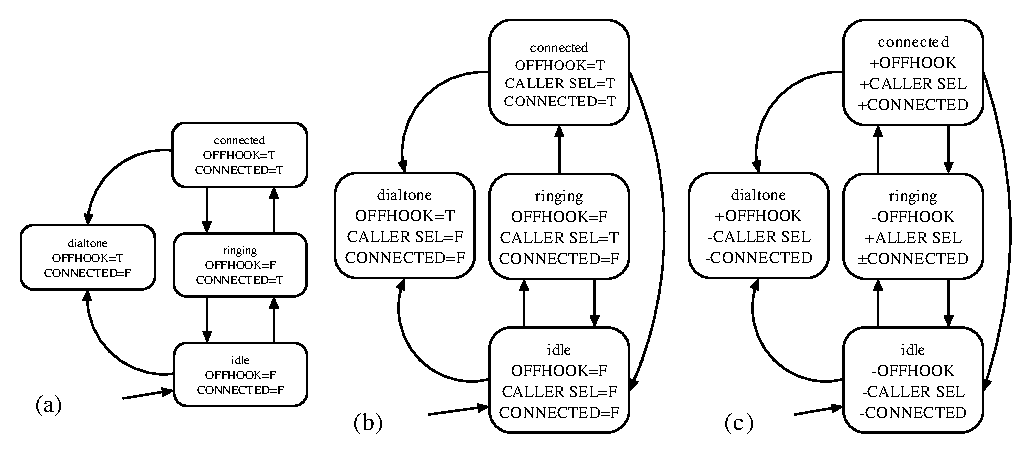
\includegraphics[scale=0.6]{merge2.eps}
\caption{(a) Viewpoint of Callee1; (b) Viewpoint of Callee2; (c)
Merger of Two Viewpoints} \label{fig:Example}
\end{figure}
Integrating multiple models is complicated when inconsistent
information exists among models. We here do this as follows:
\begin{itemize}
\item Choose the underlying logic QCTL for the merged model.
\item Choose signature maps, which stipulate the relationships of
items between the merged model and the corresponding source
models, such as states' names and propositional variables in
states. We adopt the similar principle in~\cite{Merging}.
\item
Choose the measure of handling the inconsistencies existing among
models. Optimistically, we argue that some conflicting viewpoints on
the system do not exclude each other, for instance, each model does
not deny the existence of transitions that it does not describe.
This argument, we think, is appropriate for evolving specifications,
especially in the early stage of the development.
\end{itemize}
Fig.4(c) shows the resulting paraKripke model.

Despite conflicting viewpoints on the system, we can verify some
temporal properties of the phone system. The representational
examples include:\small

\noindent1. $\texttt{A}\Box
(\texttt{CONNECTED}\rightarrow\texttt{E}\bigcirc(\neg\texttt{OFFHOOK}))\
\ \ $ ``if you are connected, you can hang up."

\noindent2.
$\texttt{A}\Box(\neg\texttt{CALLER\_SEL}\rightarrow\neg\texttt{CONNECTED})\
$ ``if none is selected, you cannot be connected."

 \noindent3.
$\texttt{A}\Box(\neg\texttt{OFFHOOK}\rightarrow\neg\texttt{CONNECTED})\
\ \ \ \ \ \ \ \ $ ``if you hang up, you are disconnected".
\normalsize

According to Definition~\ref{MC:metho}.1, we can easily ensure
that the first property is satisfiable in the merged model, that
is, Fig.4(c) is a paraKripke model of the first property. The rest
of the three properties is more interesting. The second property
is not expressible in callee1, but callee1 can have this property
as long as it accepts the definitions in callee2 for CALLER\_SEL,
which callee1 does not describe. Consider the third, from
Fig.4(c), we know the merged model satisfies the property. Just on
this property are callee1 and callee2 conflicting. Note that the
listed properties are simple, therefore, we do not explicitly
explain the details of deriving the three properties from
Fig.4(c). Though this example mentioned above is small and rather
artificial, it suffices for illustrating the type of reasoning
under inconsistency.

\section{Concluding remarks}

In this paper we presented a novel notion of paraKripke model
based on QCTL, which grasps the essential idea behind QCTL. The
methodology of checking whether a paraKripke structure is a
paraKripke model of a formula in QCTL, is deep investigated.
Further, we described the implementation of the algorithm for
model checking over QCTL.

However, it is inadequate job. We need to continue our work in the
following directions. First, We intend to conduct a series of
nontrivial case studies, showing the proposed framework makes
developers more efficient and more innovative in the continually
evolving development process, such as requirements engineering.
Further, our aim is not to replace the established approach of
handling inconsistencies existing in the life cycle of software
development. We plan to integrate the automated tools based on
paraconsistent logics  with the early work by Hunter, Finkelstein,
et al.


\begin{thebibliography}{10} \label{biblo}

\bibitem{MC} E. Clarke, O. Grumberg, and D. Peled. \emph{Model Checking}. MIT Press, 1999.

\bibitem{spin} G. J. Holzmann. The model checker SPIN. \emph{IEEE Transactions on Software
Engineering,} 23(5): 279, 1997.

\bibitem{VIS}  R. K. Brayton, G. D. Hachtel, F. Somenzi. Vis: A system for verification and
synthesis. \emph{Proceedings of the Computer Aided Verification
Conference}, 428-432, 1996.

\bibitem{Incon} B. A. Nuseibeh, C. Ghezzi. Introducation to the
issue on managing inconsistency in software development.
\emph{IEEE Transactions on Software Engineering}, 24(11):
906-1001, 1998.

\bibitem{Incon1} A. Russo, B. Nuseibeh, S. Easterbrook.
Making Inconsistency Respectable in Software Development.
\emph{Journal of Systems and Software,} 58(2): 171-180, 2001.

\bibitem{Handle1} A. Finkelstein, A. Hunter, D. Gabbay,  et al.
Inconsistency handling in multi-perspective specifications.
\emph{IEEE Transactions on Software Engineering,} 20: 569--578,
1994.

\bibitem{Hunter1} A. Hunter, B. Nuseibeh. Managing inconsistent specification: Reasoning, analysis
and action. \emph{ACM Transaction on Software Engineering and
Methodology,} 7: 335- 367, 1998.

\bibitem{Formal} N. C. da Costa. On the theory of inconsistent formal system. Notre Dame Journal
of Formal Logic, 15: 497-510, 1974.

\bibitem{MVProver1} R. H\"{a}hnl. \emph{Automated Deduction in Multiple-Valued
Logics,} Volume 10 of \emph{International Series of Monographs on
Computer Science}. Oxford University Press, 1994.

\bibitem{P.Godefroid} G. Bruns, P. Godefroid. Generalized model
checking: Reasoning about partial state spaces. \emph{Proc of
International Conference on Concurrency Theory, LNCS,} 1877:
168-182, 2000.

\bibitem{Para1} C. Mortensen, D. Bantens, G. Priest, and J. P. V.
Bendegem. \emph{Frontiers of Paraconsistent Logics.} King's
College Publications, 2000.

\bibitem{Para2} I. D. Ottaviano. On the development of
paraconsistent logic and da Costa's work. \emph{Journal of
Non-Classical Logic,} 7: 9-72, 1990.

\bibitem{QZ} R. Miarka. \emph{Inconsistent and Underdefinedness in Z
specification}. Phd thesis, The University of Kent, 2002.

\bibitem{kri1} E. A. Emerson.
Temporal and modal logic. \emph{Handbook of theoretical computer
science} (J. V. Leeuwen, eds.), Elseier Science Publisher B.V.,
1990.

\bibitem{TL} A. Pnueli, Z. Manna. Verification of concurrent
programs: The temporal framework. \emph{The correctness Problem in
Computer Science} (R. S. Boyer and J. S. Moore, editors), 215-273,
Acamemic Press, 1981.

\bibitem{ALG1} E. M. Clarke, E. A. Emerson. Design and synthesis of
synchronization skeletons using branching temporal logic.
 \emph{Lecture Notes in Computer Science}, 131: 52-71.  1981.

\bibitem{Merging} M. Sabetzadeh, S. Easterbrook.
An Algebraic Framework for Merging Incomplete and Inconsistent
Views. Technical Report CSRG-496, University of Toronto, 2004.

\end{thebibliography}

\end{document}
